\documentclass[12pt]{article}
\usepackage{times} 			% use Times New Roman font
\usepackage{longtable}
\usepackage[margin=1in]{geometry}   % sets 1 inch margins on all sides
\usepackage{hyperref}               % for URL formatting
\usepackage[pdftex]{graphicx}       % So includegraphics will work
\setlength{\parskip}{1em}           % skip 1em between paragraphs
\usepackage{indentfirst}            % indent the first line of each paragraph
\usepackage{datetime}
\usepackage[small, bf]{caption}
\usepackage{listings}               % for code listings
\usepackage{xcolor}                 % for styling code
\usepackage{multirow}
\usepackage{float}
\usepackage{enumitem}
\usepackage{nameref}

%New colors defined below
\definecolor{backcolour}{RGB}{246, 246, 246}   % 0xF6, 0xF6, 0xF6
\definecolor{codegreen}{RGB}{16, 124, 2}       % 0x10, 0x7C, 0x02
\definecolor{codepurple}{RGB}{170, 0, 217}     % 0xAA, 0x00, 0xD9
\definecolor{codered}{RGB}{154, 0, 18}         % 0x9A, 0x00, 0x12

%Code listing style named "gcolabstyle" - matches Google Colab
\lstdefinestyle{gcolabstyle}{
  basicstyle=\ttfamily\small,
  backgroundcolor=\color{backcolour},   
  commentstyle=\itshape\color{codegreen},
  keywordstyle=\color{codepurple},
  stringstyle=\color{codered},
  numberstyle=\ttfamily\footnotesize\color{darkgray}, 
  breakatwhitespace=false,         
  breaklines=true,                 
  captionpos=b,                    
  keepspaces=true,                 
  numbers=left,                    
  numbersep=5pt,                  
  showspaces=false,                
  showstringspaces=false,
  showtabs=false,                  
  tabsize=2
}

\lstset{style=gcolabstyle}      %set gcolabstyle code listing

% to make long URIs break nicely
\makeatletter
\g@addto@macro{\UrlBreaks}{\UrlOrds}
\makeatother
%\newcommand{\code}[1]{\Colorbox{mygray}{\lstinline|#1|}}
% for fancy page headings
\usepackage{fancyhdr}
\setlength{\headheight}{13.6pt} % to remove fancyhdr warning
\pagestyle{fancy}
\fancyhf{}
\rhead{\small \thepage}
\lhead{\small HW2, Adeniran}  % EDIT THIS, REPLACE # with HW number
\chead{\small CS 532, Spring 2021} 

%-------------------------------------------------------------------------
\begin{document}

\begin{centering}
{\large\textbf{HW 2 - Web Archiving}}\\ % EDIT THIS
                                % REPLACE # with HW num and ADD title
Adeniran Adeniyi\\                     % EDIT THIS
Sunday, Feb 28th 2021  by 11:59pm\\                      % EDIT THIS
\end{centering}

%-------------------------------------------------------------------------

% The * after \section just says to not number the sections

\section*{Q1}

\emph{Collect 1000 unique links from tweets in Twitter.
}
\newline
\emph{There are several steps involved in this:}
\newline
% \par\null\par
% \medskip
% \bigskip

\begin{itemize}
    \item Obtain a Twitter Developer Account, create a standalone app in the Developer Portal, and generate consumer keys (API key and secret) and authentication tokens (access token and secret) -- you should have done this in HW0
        \begin{list}{$\circ$}
            \item \href{https://piazza.com/class/khuxxbpeiesu2?cid=113}{thread in Piazza related to this}
        \end{list}
    \item Write a Python program that collects links shared in tweets.
        \begin{list}{$\circ$}
            \item exclude links from the Twitter domain (twitter.com)
        \end{list}
    \item Resolve all URIs to their final target URI (i.e., the one that responds with a 200) -- some may be shortened links (dlvr.it, bit.ly, etc.)

    \item Verify that the final URIs are unique.
        \begin{list}{$\circ$}
            \item if after this step, you don't have 1000 unique URIs, go back and gather more until you are able to get to 1000 unique URIs
        \end{list}
    \item Save this collection of links and upload it to your repo in GitHub -- we'll use it again in HW3
        
\end{itemize}
\emph{Collecting Links in Tweets}
\newline
\emph{There are several Twitter API wrappers available:}
\begin{itemize}
    \item \href{https://www.tweepy.org/}{Tweepy} -used in the example \href{https://github.com/cs432-websci-master/public/blob/main/spr21/collect-tweets.py}{collect-tweets.py} that was provided in HW0
        \begin{list}{$\circ$}
            \item 
                \href{http://docs.tweepy.org/en/latest/getting_started.html#introduction}{Tweepy documentation}
            \item 
                \href{https://docs.tweepy.org/en/v3.10.0/cursor_tutorial.html}{Cursor Tutorial}
            \item 
                \href{https://docs.tweepy.org/en/v3.10.0/api.html#search-methods}{Search Method}
            \item                                                   
                \href{https://www.geeksforgeeks.org/python-status-object-in-tweepy/}{Python - Status object in Tweepy}
            \item 
                \href{https://developer.twitter.com/en/docs/twitter-api/v1/data-dictionary/object-model/tweet}{Tweet Object} -Twitter API data structure returned
        \end{list}
\end{itemize}
\emph{There are many other similar resources available on the web}
\newline
\emph{Note that you'll likely need to collect more than 1000 links initially to get 1000 unique links.}
\newline
\emph{There are rate limits associated with different types of API calls to Twitter. The search API has a larger limit than the streaming API, so I suggest using that. Choose a few keywords and use the search API to collect links for each of those keywords. Use keywords that you might actually search for (ex: coronavirus, election, vaccine) rather than "stopwords" (ex: test, the, tweet).}
\newline
\emph{I've provided starter code, \href{}{collec-links-cursor.py} for collecting links from Twitter using the tweepy library.}

\begin{itemize}
    \item accepts a command-line parameter with the search term and uses "coronavirus" if no term is provided
    \item uses Cursor() and the search API to search for English language tweets containing the given search term
    \item attempts to collect 1200 links
        \begin{list}{$\circ$}
            \item if you get fewer than 1200 links and see Tweepy Error: Twitter error response: status code = 429 at the end of your file, you've hit the rate limit, so wait 15 minutes and try again 
\item you may want to reduce the number of links that are collected and use multiple search terms so that you can space out the requests
        \end{list}
    \item prints the URIs to stdout
    \item does not exclude links containing twitter.com -- you should add code to do this
    \item you will need to supply your Twitter API consumer\_key and consumer\_secret

\end{itemize}
\begin{lstlisting}[numbers=none]
    % python3 collect-links-cursor.py archive > links.txt
\end{lstlisting}
\emph{This will run the program with the search term "archive" and write the output to the file links.txt.}
\newline
\emph{If you find a link you consider to be inappropriate for any reason, just discard it and get some more links.}
\newline
\newline
\emph{Resolve URIs to Final Target URI}
\newline
\newline
\emph{Many of the links that you collect will be shortened links (dlvr.it, bit.ly, buff.ly, etc.). We want the final URI that resolves to an HTTP 200 (not a redirection). For example:}
\newline
\begin{lstlisting}[numbers=none]
$ curl -IL --silent https://t.co/DpO767Md1v | egrep -i "(HTTP/1.1|HTTP/2|^location:)"
HTTP/2 301
location: https://goo.gl/40yQo2
HTTP/2 302
location: https://soundcloud.com/roanoketimes/ep-95-talking-hokies-recruiting-one-week-before-signing-day
HTTP/1.1 200 OK
\end{lstlisting}
\emph{We want https://soundcloud.com/roanoketimes/ep-95-talking-hokies-recruiting-one-week-before-signing-day, not https://t.co/DpO767Md1v or https://goo.gl/40yQo2}
\newline
\newline
\emph{You can either write a Unix shell script that uses curl to do this, or write a Python program using the \href{https://requests.readthedocs.io/en/master/}{requests library.}}
\emph{Save Only Unique URIs}
\newline
\newline
\emph{You can write Python code for this part, but I'd strongly recommend using the Unix tools sort and uniq. \href{https://www.linuxjournal.com/content/back-basics-sort-and-uniq}{Back to Basics: Sort and Uniq} is a nice introduction to this.}


\subsection*{\color{blue}{Answer}}
% \emph{All figures must have a caption and must be referenced in the text. Example below.}
\begin{figure}[H]
    \centering
    % trim and clip are used to crop the image, trim=left bottom right top
    % width sets max width, height will be scaled appropriately
    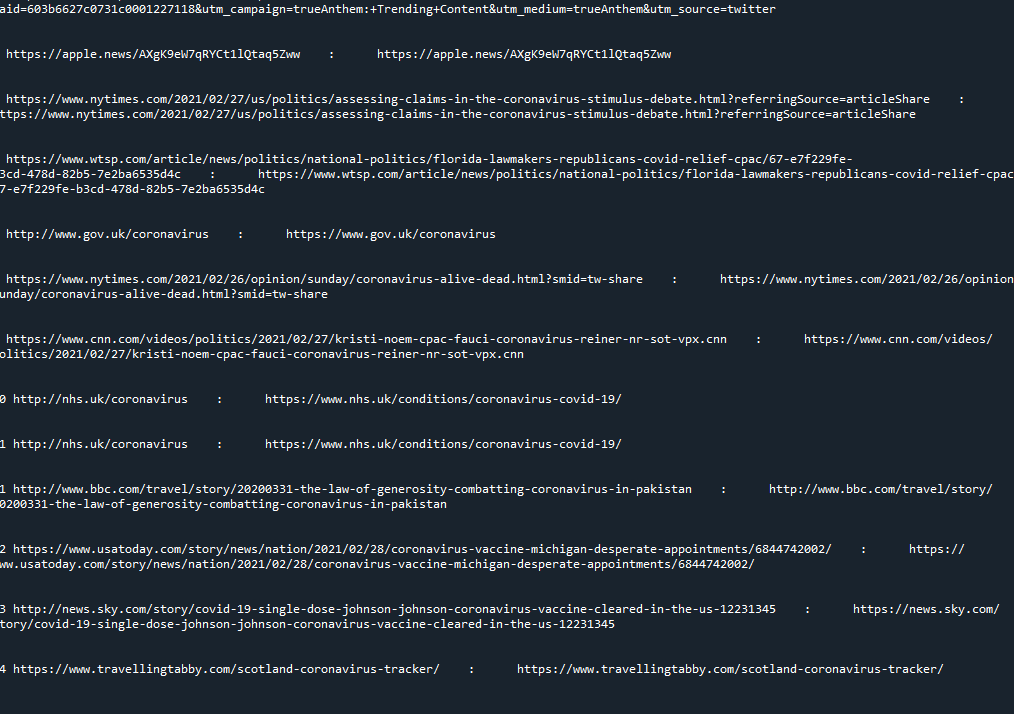
\includegraphics[trim=0 10 0 80, clip, width=\textwidth] {running.PNG}
    \caption{sample running output shows(count,URI-R gotten, resolved URI-R)}
    \label{fig:Running output}
\end{figure}
\lstinputlisting[language=Python, caption=Part of Output text file, label=dict.txt:import,firstnumber=1,firstline=1,lastline=50]{dict.txt}
\lstinputlisting[language=Python, caption=Collect-link-cursor.py, label=collect-link-cursor.py:import,firstnumber=1,firstline=1,lastline=120]{collect-links-cursor.py}
\subsection*{Discussion}

\emph{I followed these instruction below:}

\begin{itemize}
    \item Obtain a Twitter Developer Account, create a standalone app in the Developer Portal, and generate consumer keys (API key and secret) and authentication tokens (access token and secret) -- you should have done this in HW0
    \emph{\\ \\ \color{blue}{Answer:}}
    \emph{\\   I created this a while back by clicking  \href{https://developer.twitter.com/en/apply-for-access}{\color{red}{Apply for Access}} and followed the instructions. \\ \\ Here is a picture of the created account}
    \begin{figure}[H]
        \centering
        % trim and clip are used to crop the image, trim=left bottom right top
        % width sets max width, height will be scaled appropriately
        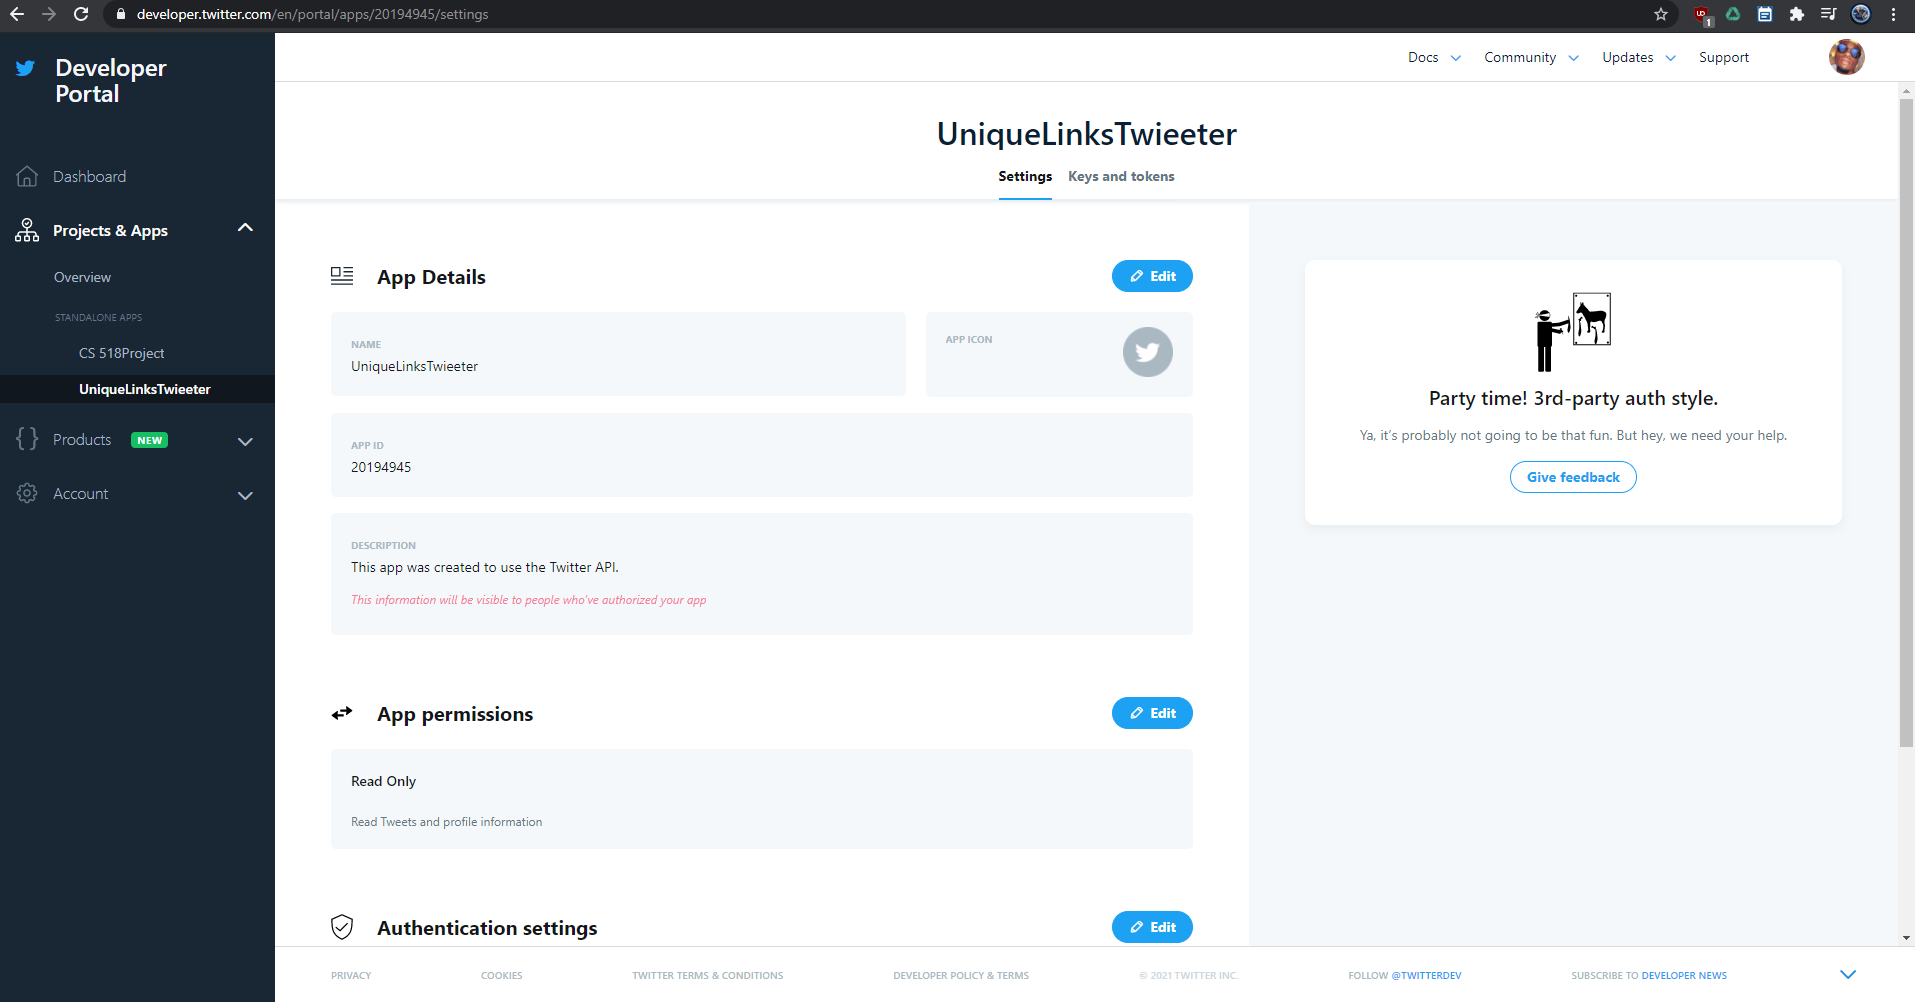
\includegraphics[trim=0 10 0 80, clip, width=\textwidth] {twiiterAccountPNG.PNG}
        \caption{Development Account and Application}
        \label{fig:Dev Account}
    \end{figure}
        
    \item Write a Python program that collects links shared in tweets.
        \begin{list}{$\circ$}
            \item exclude links from the Twitter domain (twitter.com)
        \end{list}
        \lstinputlisting[language=Python,caption=snapshot of collect-link-cursor.py, label=3snapshotcollect:import,firstnumber=23,firstline=23,lastline=33]{collect-links-cursor.py}
        \emph{\\ \\ \color{blue}{Answer:}}
        \emph{\\ \\I performed this by getting the link tweepy gave me and passed it in the resolve\_url function on line 72}
        \lstinputlisting[language=Python, label=lst:import,firstnumber=72,firstline=72,lastline=72]{collect-links-cursor.py}
        \emph{On line 24 I got the domain of the link and checked if it was had a twitter URL.\\ If it wasnt a twitter URL I saved it. Making the link fully resolved.}
    \item Resolve all URIs to their final target URI (i.e., the one that responds with a 200) -- some may be shortened links (dlvr.it, bit.ly, etc.)
        \emph{\\ \\\color{blue}{Answer:}}
        \emph{\\ \\ I first ensured that there was a 200 status code on each request performed. This can be seen in line 20}
        \lstinputlisting[language=Python, label=lst:import,firstnumber=20,firstline=20,lastline=20]{collect-links-cursor.py}
        \emph{\\In the resolve\_url function on line 24}
        \lstinputlisting[language=Python, label=lst:import,firstnumber=24,firstline=24,lastline=24]{collect-links-cursor.py}
         \emph{\\ \\This gets the full final url after following any redirection.}
        
        
    \item Verify that the final URIs are unique.
        \begin{list}{$\circ$}
            \item if after this step, you don't have 1000 unique URIs, go back and gather more until you are able to get to 1000 unique URIs
        \end{list}
        \emph{\\  \color{blue}{Answer:}}

        \lstinputlisting[language=Python,caption=snapshot of collect-link-cursor.py, label=4snapshotcollect:import,firstnumber=74,firstline=74,lastline=81]{collect-links-cursor.py}
        \emph{\\ \\ Once I received the resolved URL in line 72.\lstinputlisting[language=Python, label=lst:import,firstnumber=72,firstline=72,lastline=72]{collect-links-cursor.py} I used a dictionary data structure declared on line 59 to store url as the key of the dictionary and assigned an integer 1 to indicate that the string has been added to the dictionary blank\_dict. Subsequently when the same link is received again on line 72\lstinputlisting[language=Python, label=lst:import,firstnumber=72,firstline=72,lastline=72]{collect-links-cursor.py}, line 74\lstinputlisting[language=Python, label=lst:import,firstnumber=74,firstline=74,lastline=74]{collect-links-cursor.py} reduce the count value by one. count variable on declared on line 55\lstinputlisting[language=Python, label=lst:import,firstnumber=55,firstline=55,lastline=55]{collect-links-cursor.py} tracks the number of links resolved. In line 84\lstinputlisting[language=Python, label=lst:import,firstnumber=84,firstline=84,lastline=84]{collect-links-cursor.py} , ensures count gets to run 1000 times as declared on line 54.\lstinputlisting[language=Python, label=lst:import,firstnumber=54,firstline=54,lastline=54]{collect-links-cursor.py}}
    \item Save this collection of links and upload it to your repo in GitHub -- we'll use it again in HW3
        \emph{\\ \\ \color{blue}{Answer:}}

        \lstinputlisting[language=Python,caption=snapshot of collect-link-cursor.py label=5snapshotcollect:import,firstnumber=98,firstline=98,lastline=101]{collect-links-cursor.py}
        \emph{First swapped the dictionary keys and values respectively. This can be seen on line 95. \lstinputlisting[language=Python, label=lst:import,firstnumber=95,firstline=95,lastline=95]{collect-links-cursor.py} Then In line 98  \lstinputlisting[language=Python, label=lst:import,firstnumber=98,firstline=98,lastline=98]{collect-links-cursor.py} I named the file dict.txt, including the file path where the file should be stored. Finally deposted the result for each values to the text file line by line.
        \lstinputlisting[language=Python, label=lst:import,firstnumber=101,firstline=101,lastline=101]{collect-links-cursor.py} }
        
\end{itemize}
\section*{Q2}
\emph{Download the \href{http://www.mementoweb.org/guide/quick-intro/}{TimeMaps} for each of the unique URIs from Q1 using the ODU Memento Aggregator, MemGator. (Save the TimeMaps and upload them to your GitHub repo -- you'll also use these for Q3.) \\ \\
You may use \href{https://memgator.cs.odu.edu/}{https://memgator.cs.odu.edu} for limited testing, but do not request all of your 1000 TimeMaps from memgator.cs.odu.edu. \\ \\
There are two options for running MemGator locally:}
\begin{itemize}
    \item Install a stand-alone version of MemGator on your own machine, \\see \href{https://github.com/oduwsdl/MemGator/releases}{https://github.com/oduwsdl/MemGator/releases}
        \begin{list}{$\circ$}
            \item This was described in     \href{https://github.com/cs432-websci-master/public/blob/main/spr21/HW0.md#memgator}{HW0}
        \end{list}

    \item Install \href{https://www.docker.com/products/docker-desktop}{Docker Desktop} and run MemGator as a Docker Container, \\see notes at \href{https://github.com/oduwsdl/MemGator/blob/master/README.md}{https://github.com/oduwsdl/MemGator/blob/master/README.md}
\end{itemize}

\emph{Important: Downloading TimeMaps requires contacting several different web archives for each URI-R. This process will take time. Look at MemGator options and figure out how to process the output before running the entire process. You might want to get JSON output, or you might want to limit to the top k archives (especially if there's one that's currently taking a long time to return). \\ \\
Once you have downloaded and saved all of the TimeMaps, you will use them to analyze how well the URIs you collected are archived.
\\ \\
Create a table showing how many URI-Rs have certain number of mementos. For example}

\begin{center}
\begin{longtable}{|l|l|}
\caption{A sample long table.} \label{tab:long} \\

\hline \multicolumn{1}{|c|}{\textbf{Mementos}} & \multicolumn{1}{c|}{\textbf{URI-Rs}}  \\ \hline 
\endfirsthead

\multicolumn{2}{c}%
{{\bfseries \tablename\ \thetable{} -- continued from previous page}} \\
\hline \multicolumn{1}{|c|}{\textbf{Mementos}} & \multicolumn{1}{c|}{\textbf{URI-Rs}}  \\ \hline 
\endhead

\hline \multicolumn{2}{|c|}{{Continued on next page}} \\ \hline
\endfoot

\hline \hline
\endlastfoot
0        & 750    \\
1        & 150    \\
2        & 50     \\
5        & 47     \\
57        & 3     \\  
\end{longtable}
\end{center}
\emph{If you are using LaTeX, you should create a \href{https://www.overleaf.com/learn/latex/tables}{LaTeX table} -- don't submit a spreadsheet or image of a table created in something else. If you are using Markdown, view the source of this file for an example of how to generate a table. \\ \\ \\What URI-Rs had the most mementos? Did that surprise you?}
\subsection*{\color{blue}{Answer}}
\lstinputlisting[language=Python,caption=runShell.ps1, label=runShell.ps1:import,firstnumber=1,firstline=1,lastline=12]{runShell.ps1}
\lstinputlisting[language=Python,caption=the processing data file using analyze.py, label=analyze.py:import,firstnumber=1,firstline=1,lastline=143]{analyze.py}
\begin{figure}[H]
            \centering
            % trim and clip are used to crop the image, trim=left bottom right top
            % width sets max width, height will be scaled appropriately
            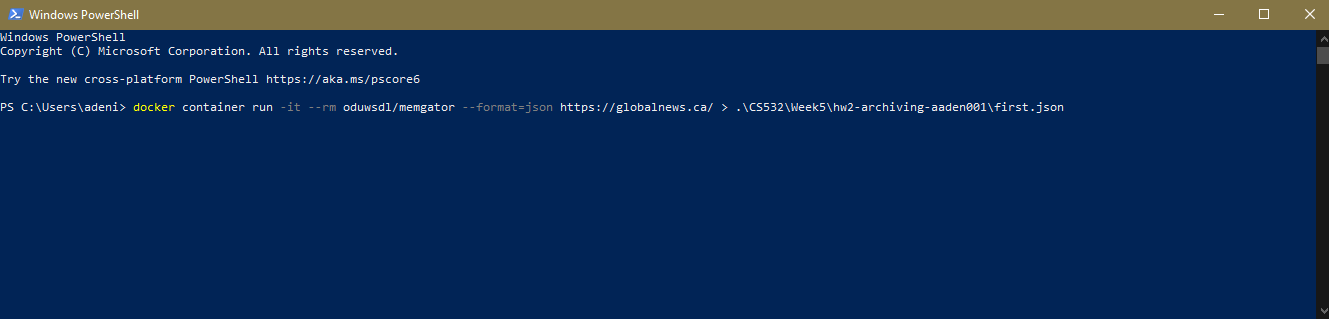
\includegraphics[trim=0 0 0 0, clip, width=\textwidth] {testCommand.PNG}
            \caption{test command in power shell for single output}
            \label{fig:Q2Ans}
        \end{figure}
\subsection*{Discussion}
\emph{I followed these instruction below:}
\begin{itemize}
    \item Run MemGator Locally using docker
        \emph{\\  \\ \color{blue}{Answer}}
        \emph{\\ \\I followed this step}
        \begin{list}{$\circ$}
            \item I Installed \href{https://www.docker.com/products/docker-desktop}{\color{red}{Docker Desktop}} and ran \href{https://github.com/oduwsdl/MemGator/blob/master/README.md#running-as-a-docker-container}{\color{red}{MemGator}} as a Docker Container, see the notes at \href{https://github.com/oduwsdl/MemGator/blob/master/README.md}{\color{red}{\\ https://github.com/oduwsdl/MemGator/blob/master/README.md}}
        \end{list}
    \item Using MemGator to download the time maps of each URL
        \emph{\\  \\ \color{blue}{Answer}}
        \emph{\\ \\I followed these steps}
        \begin{list}{$\circ$}
            \item I tested the command in line 8 of runShell.psa( \ref{runShell.ps1:import}) on Windows PowerShell \lstinputlisting[language=Python,caption=the automated command (snapshot runShell.ps1), label=1snapshotShell:import,firstnumber=8,firstline=8,lastline=8]{runShell.ps1}command line. An it produced the desired output.
            \item I Automated the process using a shell script on windows powershell as seen in Listing \ref{runShell.ps1:import} above. \\ \\ This runs the command through each line in the text file in Q1\slash dict.txt.  \\ Finally it deposits each result to a different text file. All text files are stored in Q2\slash json folder
        \end{list}
    \item Get total URI-Rs For each number of Mementos 
        \emph{\\  \\ \color{blue}{Answer}}
        \emph{\\ \\Each of the serialized text files in Q2\slash json are retrieved. This was done using analyze.py and the information was saved in the dictionary letCount see line 68 -79}
        \lstinputlisting[language=Python,caption=processes info (snapshot analyze.py), label=1snapshotShell:import,firstnumber=68,firstline=68,lastline=79]{analyze.py}
        \emph{I sorted letCount dictionary into dict1, I then parsed the sorted dictionary to a pandas DataFrame in line 90 to 95. This result is store in a csv f} \lstinputlisting[language=Python,caption=saving the table as a csv file using pandas (snapshot analyze.py), label=1snapshotShell:import,firstnumber=90,firstline=90,lastline=95]{analyze.py}
        
        \emph{
        I repeated the same process for the list MAX\_MOMENTOUS in line 104 to 106. This result is stored in a csv file. MAX\_MOMENTOUS contains the the top two URI-Rs with a Highest Momentos}
        \lstinputlisting[language=Python,caption=saving top two URIs with the highest Momentos (snapshot analyze.py), label=1snapshotShell:import,firstnumber=104,firstline=104,lastline=106]{analyze.py}
        \emph{These result can be seen on the console(\ref{fig:Q2Ans})}
        \begin{figure}[H]
            \centering
            % trim and clip are used to crop the image, trim=left bottom right top
            % width sets max width, height will be scaled appropriately
            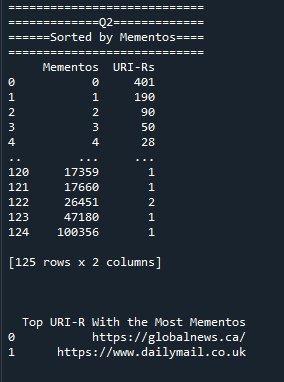
\includegraphics[trim=0 0 0 0, clip, width=\textwidth] {q2.PNG}
            \caption{Console output of Question 2 (data has be sorted in ascending order based on the number of Mementos)}
            \label{fig:Q2Ans}
        \end{figure}
    \item Create a table showing how many URI-Rs have certain number of mementos
        \emph{\\  \\ \color{blue}{Answer}}

        \begin{center}
        \begin{longtable}{|l|l|}
        \caption{A table showing Number of URI-Rs with associated to a particular number of momentos} \label{tab:long} \\
        
        \hline \multicolumn{1}{|c|}{\textbf{Mementos}} & \multicolumn{1}{c|}{\textbf{URI-Rs}}  \\ \hline 
        \endfirsthead
        
        \multicolumn{2}{c}%
        {{\bfseries \tablename\ \thetable{} -- continued from previous page}} \\
        \hline \multicolumn{1}{|c|}{\textbf{Mementos}} & \multicolumn{1}{c|}{\textbf{URI-Rs}}  \\ \hline 
        \endhead
        
        \hline \multicolumn{2}{|c|}{{Continued on next page}} \\ \hline
        \endfoot
        
        \hline \hline
        \endlastfoot
        0        & 401    \\
        1        & 190    \\
        2        & 90     \\
        3        & 50     \\
        4        & 28     \\
        5        & 23     \\
        6        & 13     \\
        7        & 11     \\
        8        & 7      \\
        9        & 14     \\
        10       & 10     \\
        11       & 9      \\
        12       & 5      \\
        13       & 5      \\
        14       & 1      \\
        15       & 2      \\
        16       & 4      \\
        17       & 1      \\
        19       & 1      \\
        20       & 3      \\
        21       & 1      \\
        22       & 2      \\
        23       & 6      \\
        24       & 2      \\
        25       & 3      \\
        27       & 1      \\
        28       & 1      \\
        29       & 3      \\
        30       & 2      \\
        31       & 2      \\
        32       & 1      \\
        33       & 1      \\
        34       & 2      \\
        35       & 1      \\
        36       & 1      \\
        39       & 1      \\
        42       & 1      \\
        43       & 2      \\
        45       & 1      \\
        46       & 1      \\
        47       & 1      \\
        48       & 1      \\
        49       & 1      \\
        50       & 1      \\
        53       & 1      \\
        54       & 1      \\
        56       & 1      \\
        57       & 2      \\
        59       & 1      \\
        60       & 2      \\
        61       & 3      \\
        62       & 1      \\
        70       & 1      \\
        71       & 2      \\
        73       & 1      \\
        80       & 1      \\
        81       & 1      \\
        82       & 1      \\
        100      & 3      \\
        110      & 1      \\
        113      & 2      \\
        122      & 1      \\
        123      & 1      \\
        127      & 1      \\
        132      & 1      \\
        136      & 1      \\
        142      & 1      \\
        143      & 1      \\
        161      & 1      \\
        169      & 1      \\
        173      & 1      \\
        174      & 1      \\
        176      & 1      \\
        181      & 1      \\
        192      & 1      \\
        195      & 1      \\
        198      & 1      \\
        216      & 1      \\
        223      & 1      \\
        225      & 1      \\
        229      & 1      \\
        233      & 1      \\
        235      & 1      \\
        236      & 1      \\
        244      & 1      \\
        245      & 2      \\
        258      & 1      \\
        284      & 1      \\
        318      & 1      \\
        319      & 1      \\
        331      & 1      \\
        334      & 1      \\
        354      & 1      \\
        357      & 1      \\
        390      & 1      \\
        392      & 1      \\
        396      & 1      \\
        412      & 1      \\
        470      & 1      \\
        525      & 2      \\
        530      & 1      \\
        540      & 1      \\
        583      & 1      \\
        635      & 1      \\
        640      & 1      \\
        1335     & 1      \\
        1448     & 1      \\
        1478     & 1      \\
        1536     & 1      \\
        1609     & 1      \\
        1824     & 1      \\
        2129     & 1      \\
        2294     & 1      \\
        2405     & 1      \\
        2843     & 1      \\
        3715     & 2      \\
        3816     & 1      \\
        4866     & 1      \\
        5717     & 1      \\
        10000    & 1      \\
        17359    & 1      \\
        17660    & 1      \\
        26451    & 2      \\
        47180    & 1      \\
        100356   & 1      \\ 
        \end{longtable}
        \end{center}
    \item \emph{What URI-Rs had the most mementos?}
        \begin{list}{$\circ$}              
                \item The URI-R with the most mementos came from \href{https://globalnews.ca/
}{\color{red}{https://globalnews.ca/}} with 100,356 mementos, followed by \href{https://www.dailymail.co.uk
}{\color{red}{https://www.dailymail.co.uk}} with 47180 mementos

        \end{list}
    \item \emph{Did that surprise you?}
        \begin{list}{$\circ$}
            \item \emph{The main reason why this link was not a surprise is because they are top news agency network. For instance globalnews.ca according to \href{https://en.wikipedia.org/wiki/Global_News}{\color{red}{https://en.wikipedia.org/wiki/Global\_News}} was founded in 1994. That enough explains the reason why the URI-R is very old.
            \\ \\ Similar case can be said for  \href{https://www.dailymail.co.uk
}{\color{red}{https://www.dailymail.co.uk} } according to \href{https://en.wikipedia.org/wiki/Daily_Mail}{\color{red}{Wikipedia}}
            }
        \end{list}
\end{itemize}


\section*{Q3}

\emph{For each of the URI-Rs from Q2 that had > 0 mementos, use the saved TimeMap to determine the datetime of the earliest memento.
\\ \\
Create a scatterplot with the age of each URI-R (days between collection date and earliest memento datetime) on the x-axis and number of mementos for that URI-R on the y-axis. For this graph, the item is the URI-R and the attributes are the estimated age of the URI-R and the number of mementos for that URI-R.
\\ \\
This scatterplot should be created using either R or Python, not Excel.
\\ \\
What can you say about the relationship between the age of a URI-R and the number of its mementos?
\\ \\
What URI-R had the oldest memento? How many URI-Rs had an age of < 1 week, meaning that their first memento was captured the same week you collected the data?}
\newline

\subsection*{\color{blue}{Answer}}
\emph{Refer to List 
\ref{analyze.py:import} for analyze.py full code}
\begin{figure}[H]
    \centering
    % trim and clip are used to crop the image, trim=left bottom right top
    % width sets max width, height will be scaled appropriately
    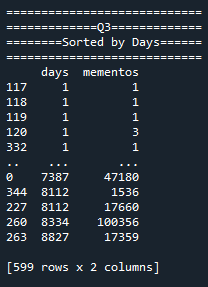
\includegraphics[trim=0 0 0 0, clip, width=\textwidth] {q3b.PNG}
    \caption{Console output of Question 3 links age to mementos amount}
    \label{fig:Q3bAns}
\end{figure}
\subsection*{Discussion}
\emph{I followed these instruction below:}
\begin{itemize}
    \item \emph{For each of the URI-Rs from Q2 that had \textless  0 mementos, use the saved TimeMap to determine the datetime of the earliest memento.}
    \emph{\\ \\Each of the serialized text files in Q2\slash json are retrieved. This was done using analyze.py and the information are saved in two dictionary daysMementos1 and daysMentos2. daysMentos1 stores the days while daysMentos2 stores the number of Mementos the URI-R has. See line 41 -49}
        \lstinputlisting[language=Python,caption=processes info (snapshot analyze.py), label=1snapshotShell:import,firstnumber=41,firstline=41,lastline=49]{analyze.py}
        \emph{I parsed these two dictionaries to a pandas DataFrame,sorted the values by the number of days in ascending order and store the result in a csv f
         in line 109 to 113. } \lstinputlisting[language=Python,caption=saving the table as a csv file using pandas (snapshot analyze.py), label=1snapshotShell:import,firstnumber=109,firstline=109,lastline=113]{analyze.py}
        \emph{These result can be seen on the console(\ref{fig:Q3bAns})}
        
    \item \emph{Create a scatterplot with the age of each URI-R (days between collection date and earliest memento datetime) on the x-axis and number of mementos for that URI-R on the y-axis. For this graph, the item is the URI-R and the attributes are the estimated age of the URI-R and the number of mementos for that URI-R.}
        \emph{\\  \\ \color{blue}{Answer}}

        \begin{figure}[H]
            \centering
            % trim and clip are used to crop the image, trim=left bottom right top
            % width sets max width, height will be scaled appropriately
            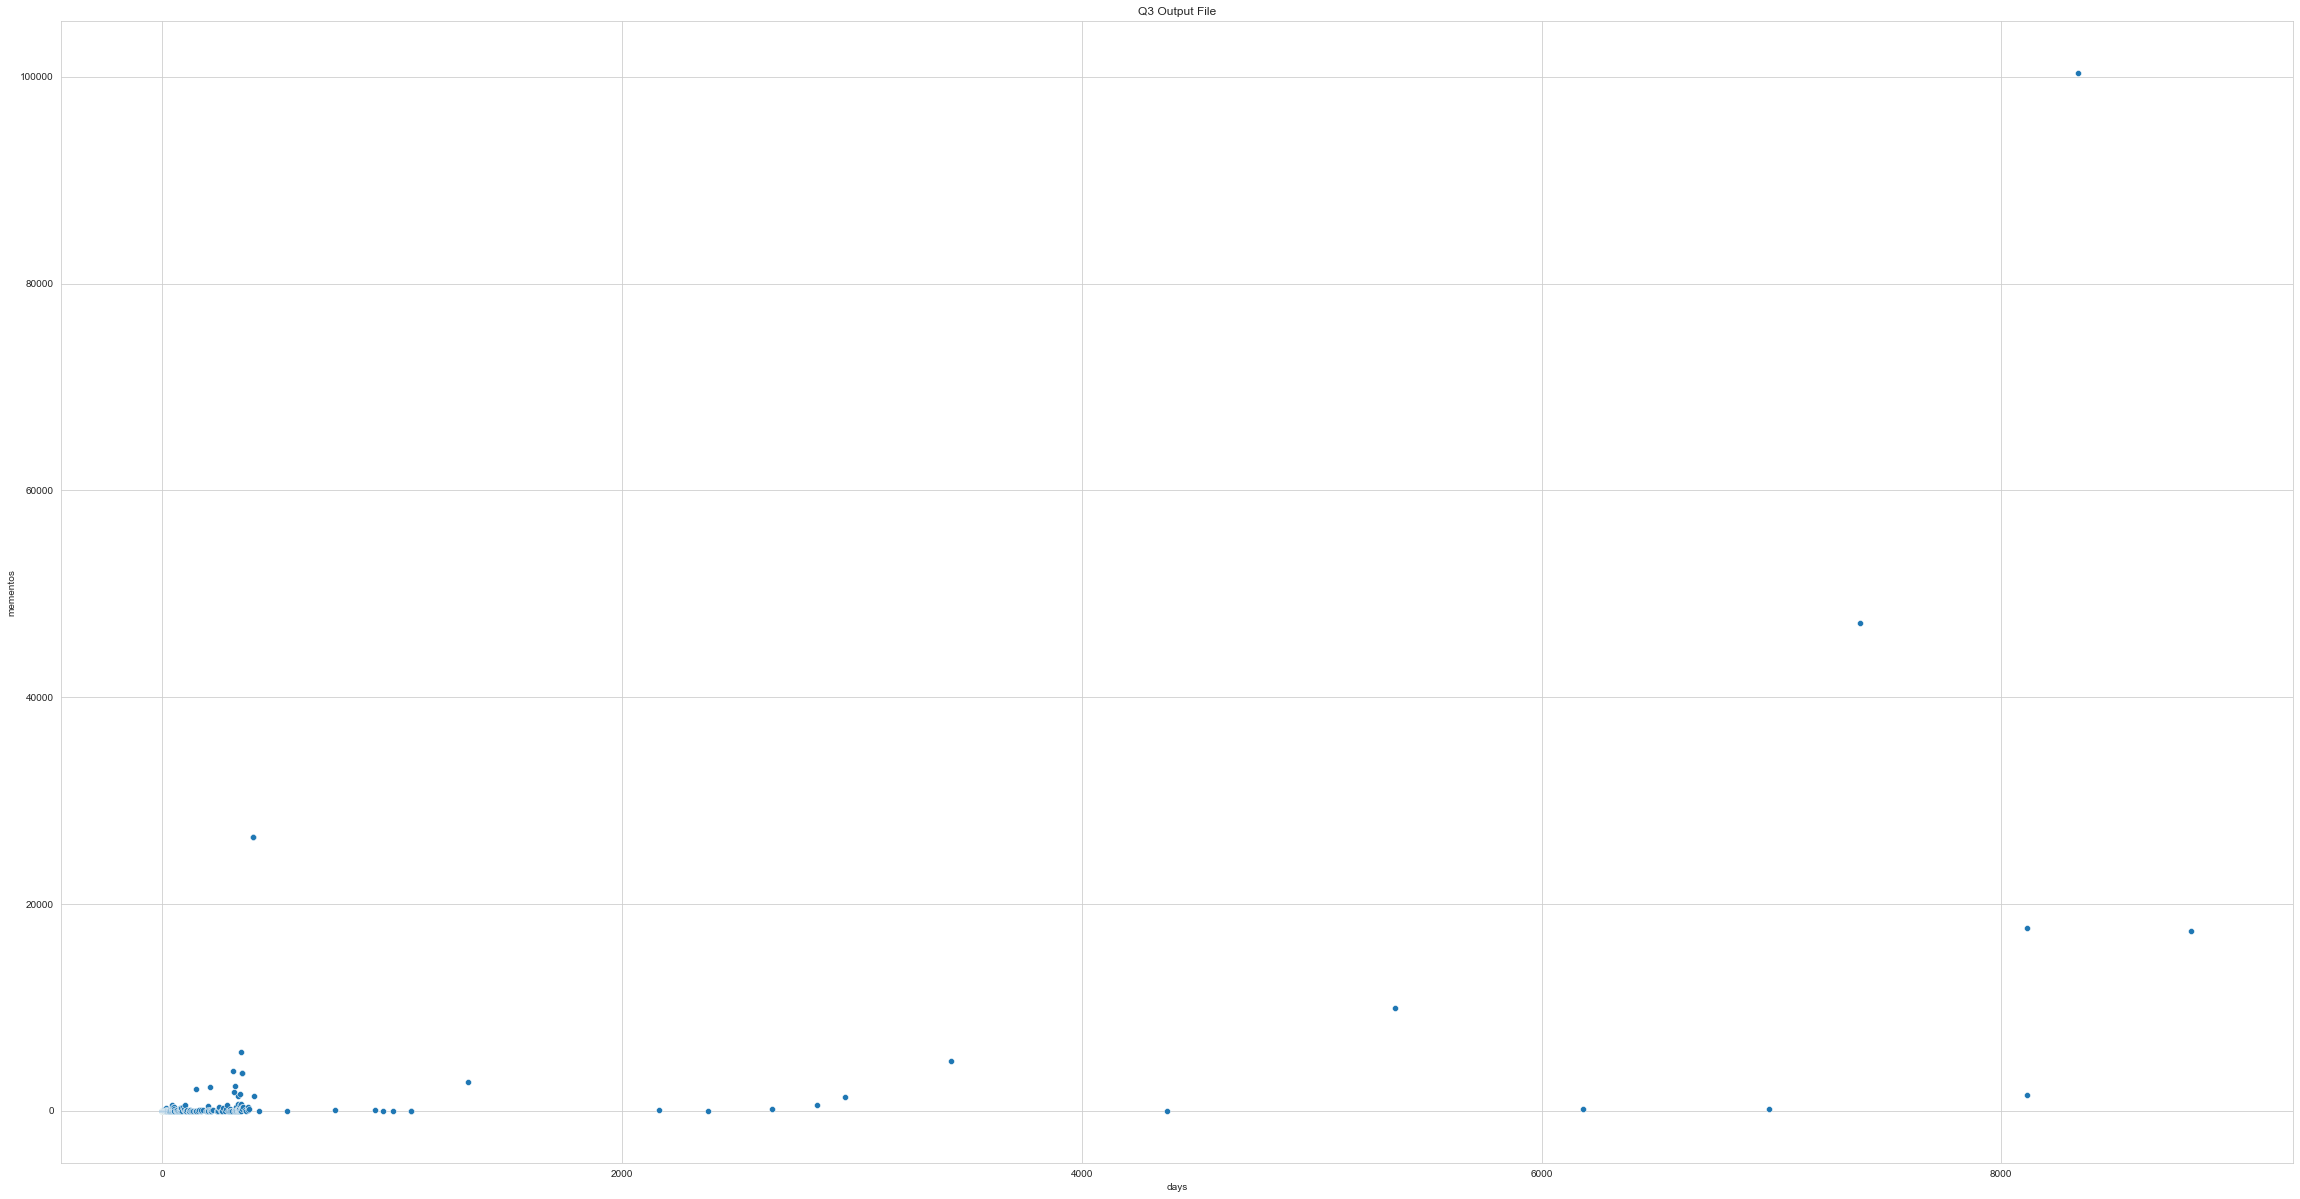
\includegraphics[trim=0 0 0 0, clip, width=\textwidth] {scatterplot.PNG}
            \caption{Console output of Question 2 (data has be sorted in ascending order based on the number of Mementos)}
            \label{fig:32Ans}
        \end{figure}  

    \item \emph{What can you say about the relationship between the age of a URI-R and the number of its mementos?}
       \emph{\\  \\ \color{blue}{Answer}}

        \begin{list}{$\circ$}              
                \item \emph{URI-Rs that tended towards zero days or less that seven day had a lower number of momentos. This means definitely correlates because these are URI-Rs that are new and therefore do not have no or less history  }
        \end{list}
    \item \emph{What URI-R had the oldest memento? How many URI-Rs had an age of < 1 week, meaning that their first memento was captured the same week you collected the data?}
        \emph{\\  \\ \color{blue}{Answer}}

        \begin{list}{$\circ$}
            \item In collecting the two top URI-Rs with the highes momentos, I compared the age of the current URI-Rs  $>$ 8112 to get the top two URI-Rs             \lstinputlisting[language=Python,caption=count momento greater than 8112 days, label=1snapshotShell:import,firstnumber=50,firstline=50,lastline=52]{analyze.py}
            \item This was done by comparing age of the URI-R(in days) \textless 7.  Using the variable old declare at zero in line 15. To increment count when this condition is satisfied.
            \lstinputlisting[language=Python,caption=count momento less than 7 days, label=1snapshotShell:import,firstnumber=54,firstline=54,lastline=55]{analyze.py}
            \begin{figure}[H]
                \centering
                % trim and clip are used to crop the image, trim=left bottom right top
                % width sets max width, height will be scaled appropriately
                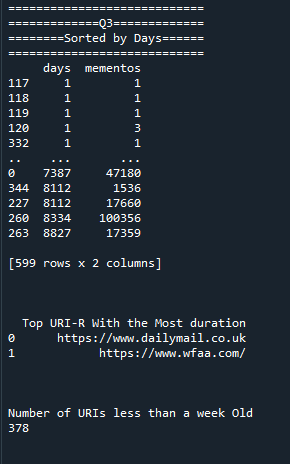
\includegraphics[trim=0 0 0 220, clip, width=\textwidth] {q3.PNG}
                \caption{Console output of Question 3 top Oldest URI-R \& URI's less that 7 days}
                \label{fig:Q3Ans}
            \end{figure}
        \end{list}
\end{itemize}


\section*{Extra Credit}
\section*{Q4 (2 points)}
\emph{Create an account at Conifer and create a collection. Archive at least 10 webpages related to a common topic that you find interesting. Make the collection public and include the link to your collection in your report.
\\ \\
Why did you choose this particular topic? Did you have any issues in archiving the webpages? Do the archived webpages look like the original webpages?
\\ \\
    After creating your collection at Conifer, download the collection as a WARC file (see \href{https://guide.conifer.rhizome.org/docs/manage-sessions/exporting-warc/}{Exporting or Downloading Content)}.
\\ \\
Then load this WARC file into \href{https://replayweb.page/}{ReplayWeb.page}, a tool from the Webrecorder Project (folks who developed Conifer). From \href{https://webrecorder.net/tools}{https://webrecorder.net/tools:}
\\ \\
ReplayWeb.page provides a web archive replay system as a single web site (which also works offline), allowing users to view web archives from anywhere, including local computer or even Google Drive. See the User guide for more info.
\\ \\
Once the WARC file has loaded, click on the "Pages" tab. Take a screenshot that includes the list of pages and the browser address bar (showing replayweb.page/?source=file%3A%2F%2F..., which indicates that the WARC file is being loaded from your local computer).
\\ \\
Then click on the "URLs" tab and choose "All URLs" from the dropdown menu. How many URLs were archived in the WARC file? How does this compare to the number of Pages?
\\ \\
Create a bar chart showing the number of URLs in the WARC file for each of the file types in the dropdown menu.
\\ \\
Which file type had the most URLs? Were you surprised by this?}
\subsection*{\color{blue}{Answer}}
\begin{itemize}
    \item \emph{Create an account at Conifer and create a collection. Archive at least 10 webpages related toa common topic that you find interesting.  Make the collection public and include the link to yourcollection in your report}
        \begin{list}{$\circ$}
            \item \href{https://conifer.rhizome.org/aaden001/crytocurrency}{\color{red}{https://conifer.rhizome.org/aaden001/crytocurrency}}
            
        \end{list}
    \item \emph{Why did you choose this particular topic? Did you have any issues in archiving the webpages? Dothe archived webpages look like the original webpages?}
        \begin{list}{$\circ$}
            \item Because crytocurrency has be a major topic on every platform today.
            \item I did not have any issues archiving the web page
            \item When I went through the archived webpages the looked very similar
        \end{list}
    \item Once the WARC file has loaded, click on the ”Pages” tab.  Take a screenshot that includes thelist of pages and the browser address bar (showing replayweb.page/?source=file
        \begin{figure}[H]
                \centering
                % trim and clip are used to crop the image, trim=left bottom right top
                % width sets max width, height will be scaled appropriately
                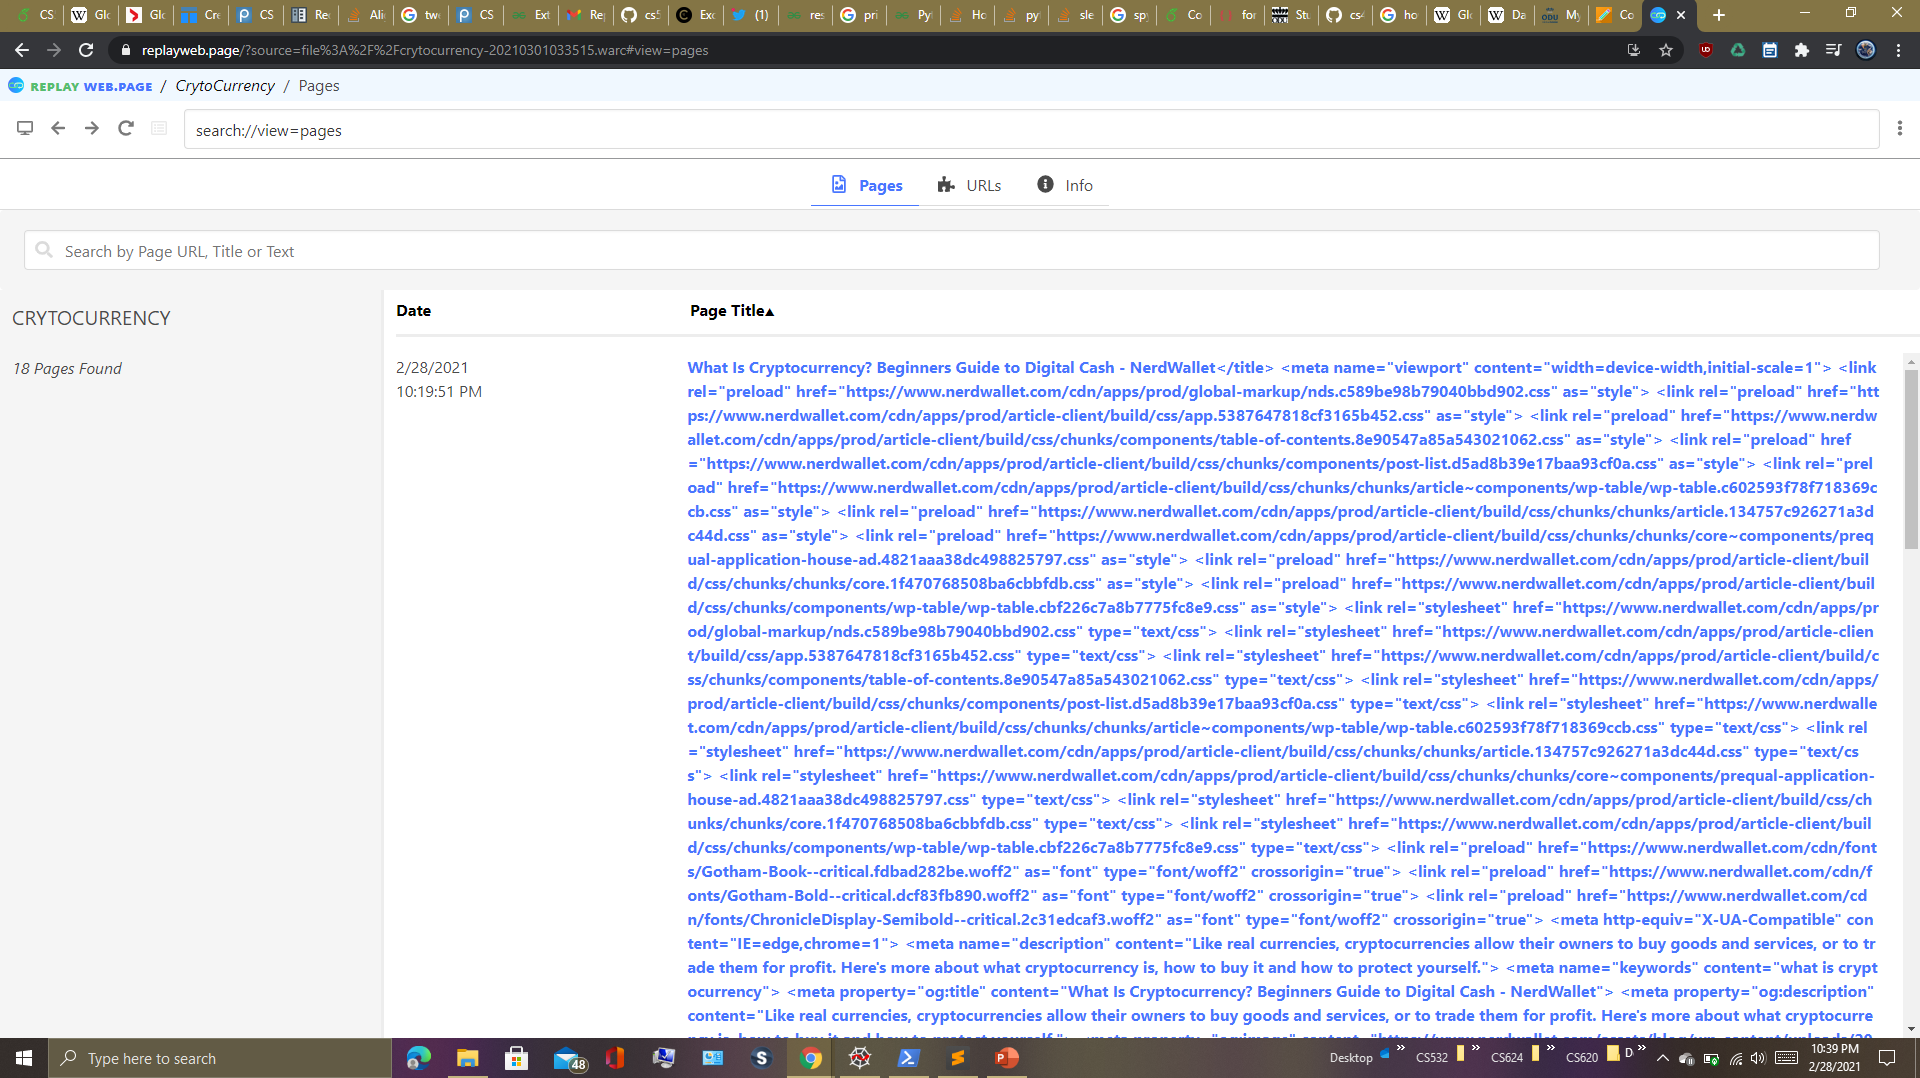
\includegraphics[trim=0 0 0 0, clip, width=\textwidth] {upload.PNG}
                \caption{File type and corresponding numbers}
                \label{fig:Q3Ans}
            \end{figure}
    \item Then  click  on  the  ”URLs”  tab  and  choose  ”All  URLs”  from  the  dropdown  menu.   How  manyURLs were archived in the WARC file? How does this compare to the number of Pages?
    \item Create a bar chart showing the number of URLs in the WARC file for each of the file types inthe dropdown menu
        \begin{list}{$\circ$}
            \item The bar chart was easily created using quickPlot.py using the code
            \lstinputlisting[language=Python,caption=count momento greater than 8112 days, label=1snapshotShell:import,firstnumber=1,firstline=1,lastline=17]{quickPlot.py}
            \begin{figure}[H]
                \centering
                % trim and clip are used to crop the image, trim=left bottom right top
                % width sets max width, height will be scaled appropriately
                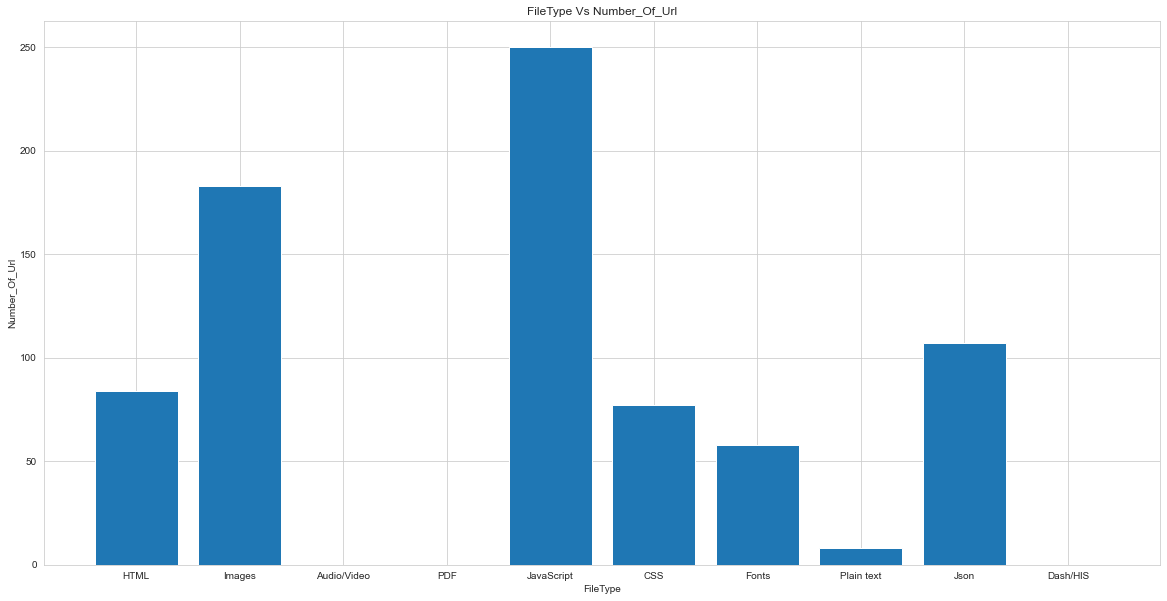
\includegraphics[trim=0 0 0 0, clip, width=\textwidth] {barchart.png}
                \caption{File type and corresponding numbers}
                \label{fig:Q3Ans}
            \end{figure}
        \end{list}
    \item Which file type had the most URLs? Were you surprised by this?
        \begin{list}{$\circ$}
            \item Java script had the most file. This is no supprise to me because a vast amount of webpages use javascripts.
        \end{list}
    
\end{itemize}
\section*{References}
\begin{itemize}
    \item { \url{https://pythonspot.com/save-a-dictionary-to-a-file/}}
    \item {\url{https://note.nkmk.me/en/python-function-return-multiple-values/}}
    \item {\url{https://www.geeksforgeeks.org/g-fact-41-multiple-return-values-in-python/}}
    \item { \url{https://www.quora.com/How-do-I-write-a-dictionary-to-a-file-in-Python}}
    \item { \url{https://www.w3schools.com/python/ref_requests_head.asp}}
    \item { \url{https://stackoverflow.com/questions/14219092/bash-script-and-bin-bashm-bad-interpreter-no-such-file-or-directory}}
    \item { \url{https://stackoverflow.com/questions/1098786/run-bash-script-from-windows-powershell}}
    \item { \url{https://www.youtube.com/watch?v=YrZLCDsh5a0}}
    \item { \url{https://stackoverflow.com/questions/45255361/raise-jsondecodeerrorexpecting-value-s-err-value}}
    \item { \url{https://wiki.python.org/moin/ForLoop}}
    \item { \url{https://stackoverflow.com/questions/53289238/convert-a-dictionary-to-dataframe-with-specified-column-names}}
    \item { \url{https://www.journaldev.com/23365/python-string-to-datetime-strptime}}
    \item { \url{https://www.geeksforgeeks.org/create-a-pandas-dataframe-from-lists/}}
    \item {\url{https://www.tablesgenerator.com/latex_tables}}
    \item {\url{https://pandas.pydata.org/pandas-docs/stable/reference/api/pandas.DataFrame.sort_values.html}}

\end{itemize}

\end{document}

